In Section~\ref{sec:metric_spaces} we show multiple ways of endowing the mapping space with a distance metric.
A common method for defining a metric in a \ac{NoC}-based system is to count the number of hops between two processors~\cite{singh2010communication,schwarzer2017symmetry}.
Indeed, this is the same as the $L_1$ (Manhattan) distance on the topology graph of the architecture.
A natural idea that arises from this is to search for \emph{compact} mappings\index{compact mappings}, i.e. mappings that take a (geometrically) small area in the chip.


\begin{figure*}[th]
	\centering
	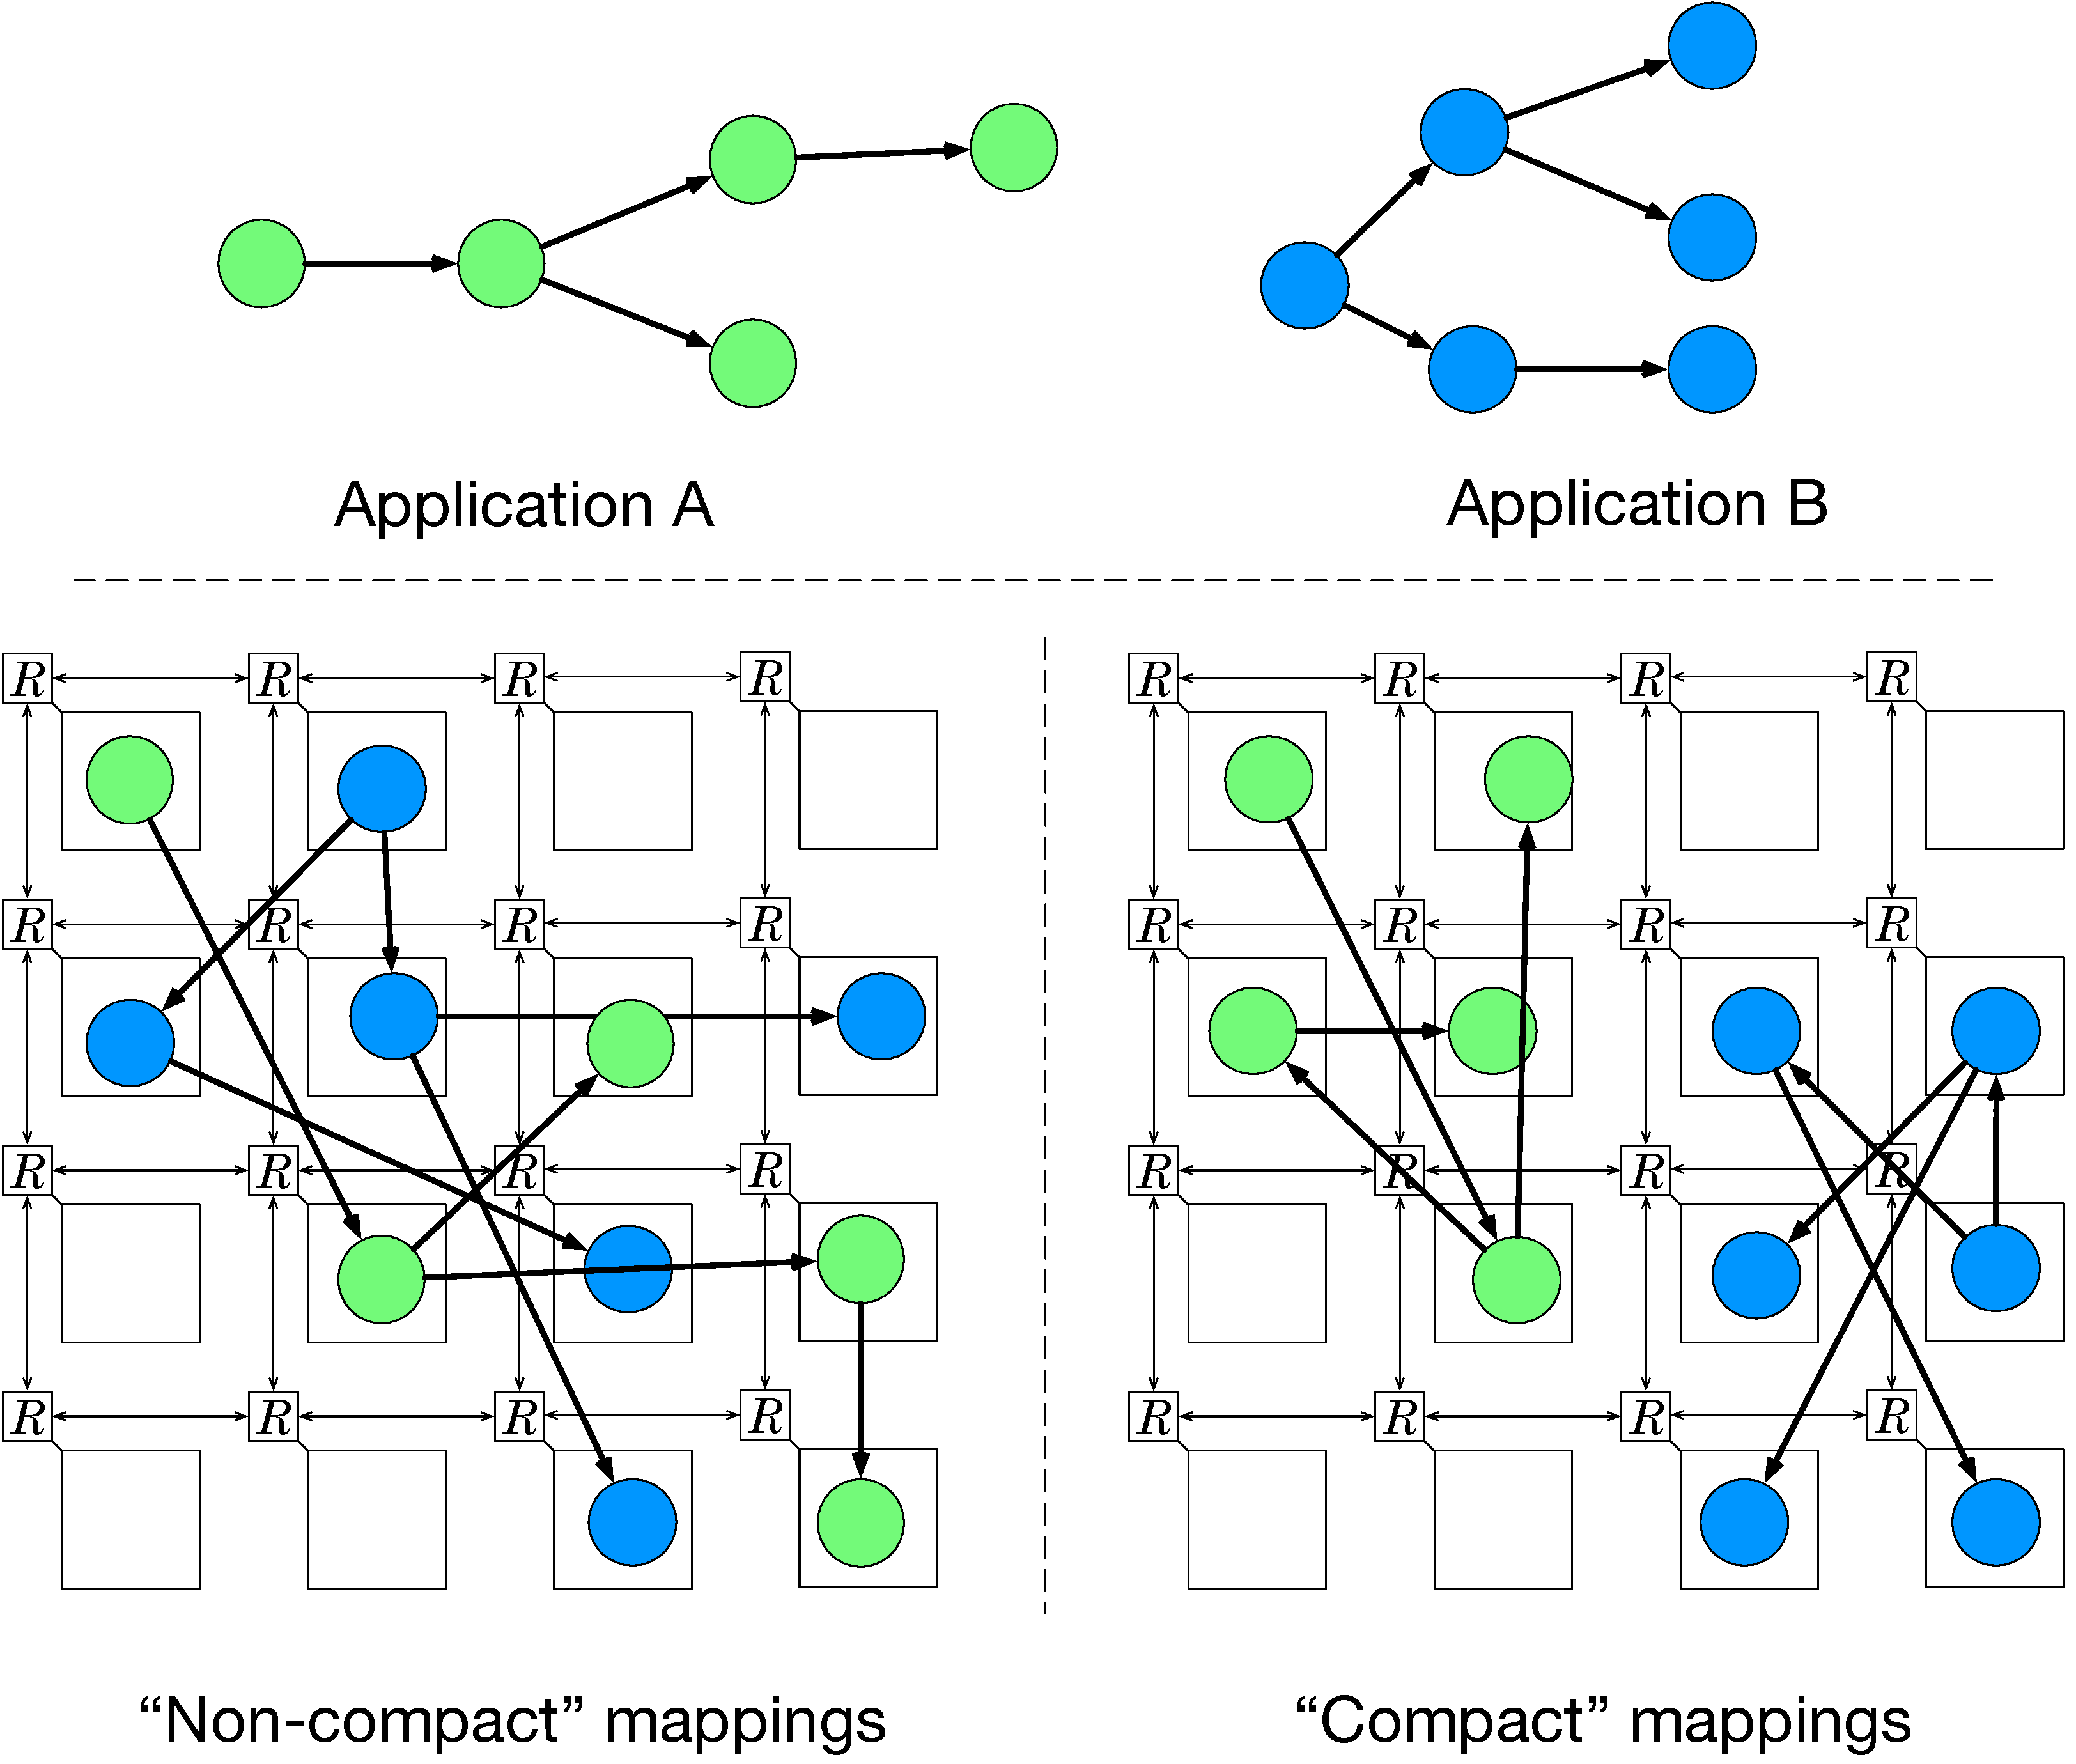
\includegraphics[width=0.6\textwidth]{figures/compact_intro.pdf}
	\caption{Equivalent mappings of two applications, one being compact and the other one not. Adapted from Figure~1 in~\cite{goens_samos19}.}
	\label{fig:compact_intro}
\end{figure*}

Figure~\ref{fig:compact_intro} illustrates well the idea of compact mappings.
It depicts two variants for mapping the two application graphs depicted in the figure.
The particular property of these two variants is that they are equivalent from the point of view of the distances:
For any two connected nodes in one of the application graphs, the node distance in terms of number of hops between both nodes is identical in both mapping variants.
Intuitively, however, the mappings on the right are preferable to those on the left. 
Does this intuition translate to actual benefits in mappings?

We used a greedy heuristic to find compact mappings in a regular mesh \ac{NoC}.
The heuristic is described in Algorithm~\ref{algo:greedy_mapping}.

\begin{algorithm}
	\caption{A greedy heuristic for low-communication mapping. Adapted from Algorithm~1 in~\cite{goens_samos19}.}
	\label{algo:greedy_mapping}
	\begin{algorithmic}[1]
	  \Input{A connected application graph $K = (V_K,E_K)$, the size of the mesh $n$,
	  a set of occupied cores $X \subseteq \{1,\ldots,n\} \times \{1 \ldots, n \} =: V_A$}
	  \Output{ A mapping $m : V_K \rightarrow V_A$ }
	  \State CurNode $\leftarrow$ RandomFrom($V_A \setminus X$)
	  \State $v_0 \leftarrow \operatorname{Root}(K)$
	  \State mapping $\leftarrow~(v_0 \mapsto \text{CurNode})$
	  \State $X \leftarrow X \cup \{ \text{CurNode} \}$
	  \For{ $e = (n_1,n_2) \in \operatorname{BreadthFirstEdgeSearch}(K)$}
		  \State CurNode $\leftarrow$ mapping($n_1$)
		  \State $d \leftarrow \min_{d = 1 \ldots n} \{a \in V_A \setminus X \mid |a - \text{CurNode}| \leq d \} \neq \emptyset $
		  \State $q \leftarrow \operatorname{RandomFrom}(\{ a \in V_A \setminus X \mid |a - \text{CurNode}| \leq d  \})$
		  \State mapping$(n_2) \leftarrow q $
		  \State $X \leftarrow X \cup \{q\}$
	  \EndFor 
	  \Return mapping
	\end{algorithmic}
  \end{algorithm}


To test this idea we used a SystemC-based \ac{NoC} simulator, Noxim~\cite{noxim}, which we modified to obtain more detailed statistics about the simulations~\cite{goens_samos19}.
In particular, we extracted the variance of the package delays in the simulation. 
We then configured Noxim to simulate a $10 \times 10$ mesh topology with xy routing and worm-hole switching. 
This choice was made to mimic the routing of commercial platforms like the Tile-Gx series from Mellanox Technologies~\cite{technologies2015-tile-gx36-processor,technologies2015-tile-gx72-processor}, or Intel's Xeon Phi~\cite{tam2018-skylake-sp} or Scalable Platform~\cite{sodani2016knights-landing}, or academic ones like OpenPiton~\cite{balkind2016-openpiton}.

We generated random task graphs with a Gilbert random graph approach (cf. Section~\ref{sec:level_graphs}) with $10$ random applications with a variable number of tasks ($4$-$6$).
For each application we then generated $100$ compact, $100$ non-compact and $100$ random mappings. 
To generate the compact and non-compact mappings we used a greedy heuristic on the distance 
\begin{figure}[h]
	\centering
   \resizebox{0.85\textwidth}{!}{\inputTikz{compact_latency.tex}}
	\caption{Comparison of latencies between compact, non-compact and random mappings. Adapted from Figure~4 in~\cite{goens_samos19}.}
	\label{fig:compact_latency}
\end{figure}

Figure~\ref{fig:compact_latency} shows the results of a comparison between compact, non-compact and random mappings. 
 These mappings were generated for $100$ different 

\begin{figure*}[th]
	\centering
	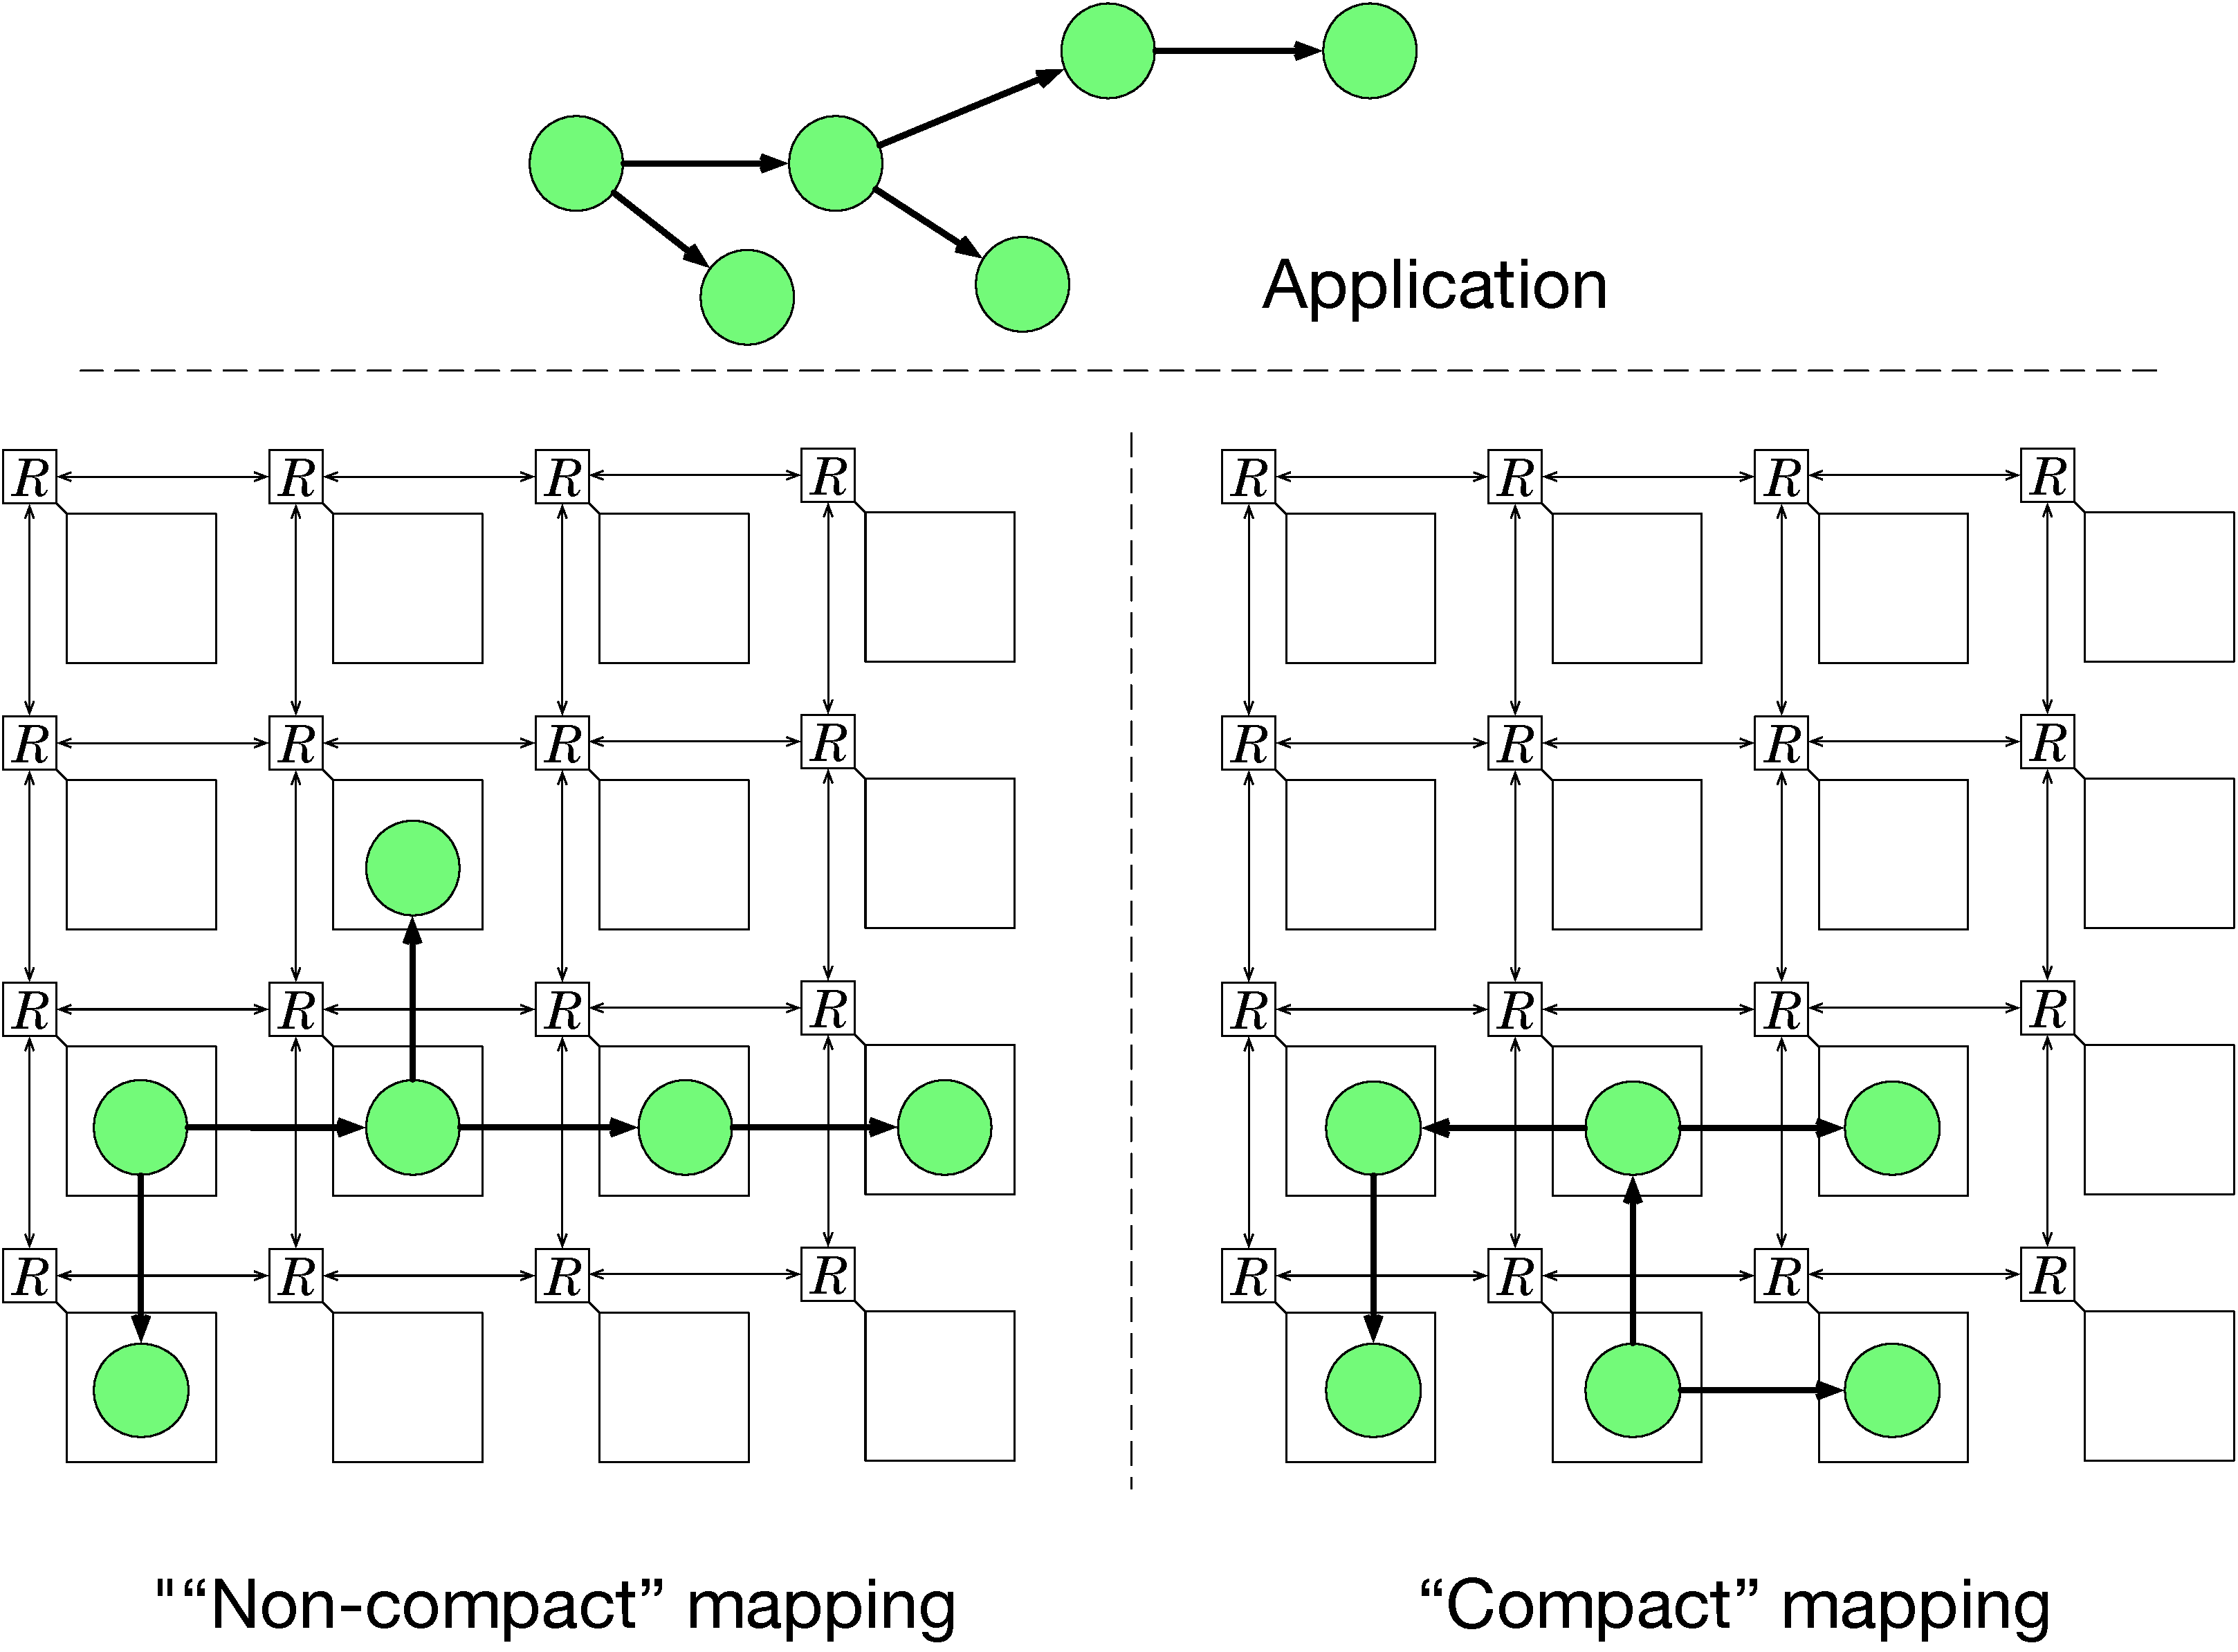
\includegraphics[width=0.6\textwidth]{figures/topology_vs_geometry.pdf}
	\caption{Two equivalent mappings that yield good performance. Adapted from Figure~2 in~\cite{goens_samos19}.}
	\label{fig:topology_vs_geometry}
\end{figure*}



\begin{figure}[h]
	\centering
   \resizebox{0.85\textwidth}{!}{\inputTikz{compact_cases.tex}}
	\caption{Comparison between compact, non-compact and random mappings running isolation or with another 9 applications. Adapted from Figure~5 in~\cite{goens_samos19}.}
	\label{fig:compact_cases}
\end{figure}